\documentclass{beamer}

\usepackage{listings}
\usepackage{tabulary}
\usepackage{amsmath}
\usepackage[utf8]{inputenc}
\usetheme{Madrid}
\setbeamersize{text margin left=0.1\textwidth,text margin right=0.1\textwidth}
\setbeamertemplate{section in toc}{\inserttocsection}
\lstset{language=python,
        keywordstyle=\color{red},
        basicstyle=\ttfamily,
        basicstyle=\small,
        frame = single,
        framexleftmargin=15pt,
        numbers=left,
        numberstyle=\small,
        numbersep=5pt,
        xleftmargin=0.05\textwidth,
        columns=fullflexible}
\definecolor{dgreen}{rgb}{0.,0.6,0.}
\definecolor{goldenrod}{rgb}{.9,0.6,0.1}

%Information to be included in the title page:
\title{Bayesian A/B Testing}
\subtitle{Conjugate Priors}
\author{Cary Goltermann}
\institute{Galvanize}
\date{2016}

 \AtBeginSubsection[]
{
  \begin{frame}
    \frametitle{Overview}
    \tableofcontents[currentsection,currentsubsection]
  \end{frame}
}

\begin{document}

\frame{\titlepage}

\begin{frame}
  \frametitle{Overview}
  \tableofcontents[]
\end{frame}

\section{Multi-Arm Bandit}
\subsection{Motivation}
\begin{frame}
  \frametitle{Motivation}
  Consider the following scenario. (You may have seen something like this before.) \vspace{2mm}
  \begin{itemize}
    \item The company you work for is testing out a new version of it's website. \pause
    \item After running an A/B test for an afternoon the new version of the site appears to performing slightly better than the old version. \pause
    \item After running the test over night, the new version of the site is performing better than the old version with a statistically significant p-value of 0.04. \pause
  \end{itemize} \vspace{3mm}

  Do you stop the test, or do you keep running it?
\end{frame}

\subsection{Exploration vs. Exploitation}
\begin{frame}
  \frametitle{Exploration vs. Exploitation}
  When we are trying to determine which option, from a potential pool, is the best option what we are faced with is an information gathering challenge. \vspace{2mm} \pause
  \begin{itemize}
    \item \textbf{\textcolor{blue}{Exploration}}: Testing out the different options (of the website), to determine how good each one is. Acquiring more knowledge about the reward associated with the options. \pause
    \item \textbf{\textcolor{blue}{Exploitation}}: Leveraging your current knowledge about the options to get the highest expected reward at that time.
  \end{itemize}
\end{frame}

\begin{frame}
  \frametitle{Traditional A/B Testing}
  A/B testing in terms of exploration vs. exploitation: \vspace{3mm}
  \begin{itemize} 
    \item Start with \textbf{pure exploration}, in which the same number of users are assigned to see each of the options. This is the testing phase. \pause
    \item Once the test is complete and some conclusion has been reached you switch to \textbf{pure exploitation}. In this phase all of the users see the version that chosen as a result of the test.
  \end{itemize}
\end{frame}

\begin{frame}
  \frametitle{Potential Inefficiencies}
  \begin{itemize}
    \item Need to wait for the experiment to conclude for certain statistical guarantees to be provided. \vspace{2mm} \pause
    \item Only after the experiment concludes can we capitalize on a potentially better option. \vspace{2mm} \pause
    \item This wastes time - and money - showing users the suboptimal site.
  \end{itemize}
\end{frame}

\begin{frame}
  \frametitle{Multi-Arm Bandit Approach}
  \begin{itemize}
    \item Show each user the site that you think is best \textbf{most} of the time. \pause (The definition of most will be dictated by your strategy. These will be discussed shortly.) \vspace{2mm} \pause
    \item As the experiment runs and you send users to different sites, update you beliefs about each site. \vspace{2mm} \pause
    \item Run until a clear best site emerges.
  \end{itemize} \vspace{3mm}

  Depending on your strategy you can balance \textbf{\textcolor{blue}{exploration}} and  \textbf{\textcolor{blue}{exploitation}} instead of having to choose either one or the other.
\end{frame}

\begin{frame}
  \frametitle{Origins}
  \begin{itemize}
    \item This problem was originally motivated from the problem that a gambler faces when deciding which slot machine (individually called one-armed bandits) to play at. \vspace{2mm} \pause
    \item Assuming that the gambler wants to be smart about their strategy they are faced, not only, with the choice of which machines to play, how many times they should play them and in what order. \vspace{2mm} \pause
    \item All they know is that each bandit will provide a reward when its lever is pulled according to its individual (and static) distribution.
  \end{itemize} \vspace{3mm} \pause

    The gambler's objective, then, is to \textbf{\textcolor{blue}{maximize}} the sum of the rewards they receive through a series of lever pulls.
\end{frame}

\begin{frame}
  \frametitle{Use Cases}
  \begin{itemize}
    \item Dynamic A/B Testing.
    \item Budget allocation amongst competing projects.
    \item Clinical trials.
    \item Adaptive routing in attempts to minimize network delays.
    \item Reinforcement learning.
  \end{itemize}
\end{frame}

\begin{frame}
  \frametitle{Fun Fact}
  \begin{block}{}
    {\large ``Originally considered by Allied scientists in World War II, it proved so intractable that, according to Peter Whittle, the problem was proposed to be dropped over Germany so that German scientists could also waste their time on it.''}
    \vspace{5mm}

    \hspace*\fill{\small--- Wikipedia}
  \end{block}
\end{frame}

\subsection{Formalization}
\begin{frame}
  \frametitle{Terminology}
  The model is given by a set of real distributions $ B = \{R_1,..., R_k\} $, where each distribution is associated with a reward delivered by one of the $ K \in \mathbb{N}^+$ levers. \vspace{3mm} \pause

  We will define the mean values associated with each of these distributions as $ \mu_1,..., \mu_k $. \vspace{3mm} \pause

  The agent plays one lever per round and observes the associated reward. The goal of the agent is to maximize the sum of the collective rewards, or alternatively, minimize the \textbf{\textcolor{blue}{regret}}.
\end{frame}

\subsection{Regret}
\begin{frame}
  \frametitle{Regret}
  The regret, $\rho$ that an agent experiences after $T$ rounds is the difference between the reward expected reward sum associated with the optimal strategy and the sum of the rewards collected.
  \begin{center}
    $\rho = T\mu^* - \sum\limits_{t=1}^{T}\hat{\rho}_t$
  \end{center}

  \begin{description}
    \item[$\mu^*$] Maximal reward mean, $\mu^* = max_k \{\mu_k\}$.
    \item[$\hat{\rho}_t$] The reward at time $t$.
  \end{description} \vspace{2mm} \pause

  \textbf{\textcolor{blue}{Regret}} can, therefore, be seen as a measure of how often you choose the suboptimal bandit. We can view this as a cost function we are trying to minimize.
\end{frame}

\begin{frame}
  \frametitle{Zero-Regret Strategy}
  A \textbf{\textcolor{blue}{zero-regret strategy}} is defined as one who's average regret per round, $\rho/T$, goes to zero in the limit where the number of rounds, $T$ goes to infinity. \vspace{6mm} \pause

  The interesting thing is that a zero-regret strategy does \textit{not} guarantee that you will never choose a suboptimal outcome. Instead it guarantees that, as you continue to play you will tend to choose the optimal outcome.
\end{frame}

\section{Strategies}
\subsection{Epsilon-Greedy}
\begin{frame}
  \frametitle{Epsilon-Greedy}
  What if we always want to explore a certain amount? \vspace{4mm}
  \pause
  \begin{itemize}
    \item \textbf{\textcolor{blue}{Explore}} with some probability $\epsilon$, often chosen as 10\%.
    \item All other times, \textbf{\textcolor{blue}{exploit}}, a.k.a. choose the bandit with the best performance so far $\rightarrow \underset{j=1,...,K}{argmax}\left \{\hat{\mu}_j(t) \right \}$.
    \begin{description} 
      \item[$\hat{\mu}_j(t)$] Our best guess for $\mu_j$ at round $t$.
    \end{description}
    \item Update our knowledge about $\mu's$ after each round.
  \end{itemize} \vspace{3mm} \pause

  Is this a zero-regret strategy?
\end{frame}

\subsection{UCB1}
\begin{frame}
  \frametitle{UCB1 (Upper Confidence Bound)}
  The UCB1 algorithm is greedily chooses the bandit with the highest $\hat{\mu}(t)$ but with a clever additional factor that automatically balances exploration and exploitation. \vspace{2mm} \pause 
  
  The choice at round $t$, after each lever is pulled once for a baseline, is made as follows: \vspace{2mm}

  \begin{center}
    $\underset{j=1,...,K}{argmax}\left \{\hat{\mu}_j(t) + \sqrt{\frac{2ln(t)}{n_j}} \right \}$
  \end{center}

  \begin{description}
    \item[$\hat{\mu}_j(t)$] Best guess for the $\mu_j$ at time $t$.
    \item[$n_j$] Number of times that bandit $j$ has been pulled.
    \item[$t$] Number of rounds that have been played in total.
  \end{description}

  Is this a zero-regret strategy?
\end{frame}

\subsection{Softmax}
\begin{frame}
  \frametitle{Softmax}
  The softmax creates a probability distribution over all the levers in proportion to how good we think each lever is. \pause

  \begin{center}
    $P_t(choosing\, bandit\, j) = \frac{e^{\hat{\mu}_j(t)/\tau}}{\sum\limits_{j=1}^{K}e^{\hat{\mu}_j(t)\tau}}$
  \end{center}

  \begin{description}
    \item[$\tau$, tau] Temperature, controls the ``randomness'' of the distribution. Usually chosen around 0.001.
  \end{description} \pause

  At each round the above distribution is sampled from and that bandit is chosen. \vspace{2mm} \pause

  A member of probability matching algorithms, so-called for their property of creating the probability distribution.

\end{frame}

\subsection{Bayesian Bandit}
\begin{frame}
  \frametitle{Bayesian Bandit}
  We can use the Bayesian beta-binomial conjugate prior techniques used to model the click-through rate in the morning exercise to as our base model for each of the bandits. \vspace{2mm}

  This is another probability matching algorithm where we have a separate model for each of the bandits. \vspace{4mm} \pause

  \textbf{\textcolor{blue}{Process}}

  \begin{itemize}
    \item Sample from the distributions for each bandit.
    \item Choose the bandit with the highest sampled $\mu$
    \item Update the distribution of the chosen bandit with the knowledge gained from choosing it.
  \end{itemize}
\end{frame}

\begin{frame}
  \frametitle{Bayesian Bandit}
  \begin{center}
    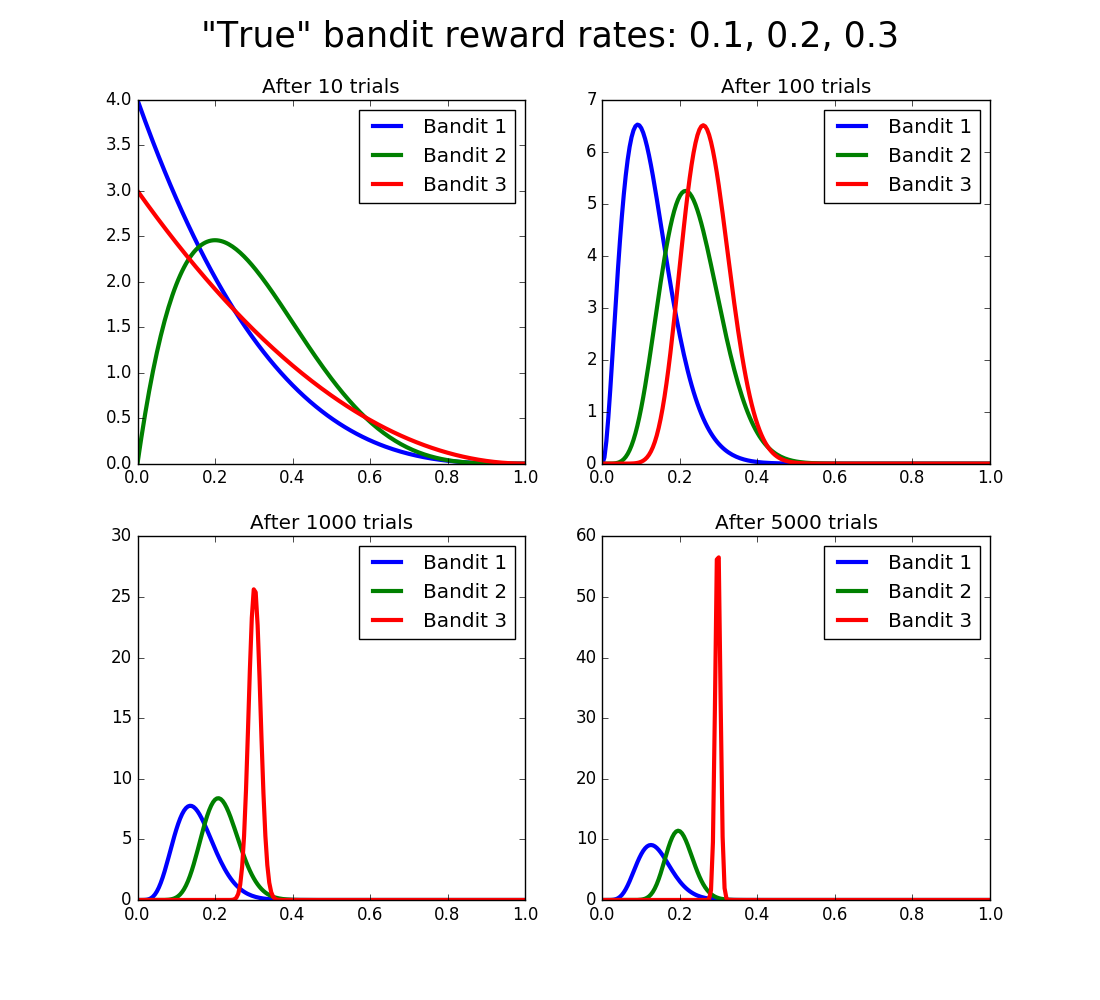
\includegraphics[width=0.8\textwidth]{images/bayesian_bandits.png}
  \end{center}
\end{frame}

\end{document}
